%%%%%%%%%%%%%%%%%%%%%%%%%%%%%%%%%%%%%%%%%
% Beamer Presentation
% LaTeX Template
% Version 1.0 (10/11/12)
%
% This template has been downloaded from:
% http://www.LaTeXTemplates.com
%
% License:
% CC BY-NC-SA 3.0 (http://creativecommons.org/licenses/by-nc-sa/3.0/)
%
%%%%%%%%%%%%%%%%%%%%%%%%%%%%%%%%%%%%%%%%%

%----------------------------------------------------------------------------------------
%	PACKAGES AND THEMES
%----------------------------------------------------------------------------------------

\documentclass[aspectratio=169, 11pt]{beamer}

\mode<presentation> {

% The Beamer class comes with a number of default slide themes
% which change the colors and layouts of slides. Below this is a list
% of all the themes, uncomment each in turn to see what they look like.

%\usetheme{default}
%\usetheme{AnnArbor}
%\usetheme{Antibes}
%\usetheme{Bergen}
%\usetheme{Berkeley}
%\usetheme{Berlin}
%\usetheme{Boadilla}
%\usetheme{CambridgeUS}

\usetheme[progressbar=frametitle]{metropolis}
%\usetheme{Copenhagen}
%\usetheme{Darmstadt}
%\usetheme{Dresden}
%\usetheme{Frankfurt}
%\usetheme{Goettingen}
%\usetheme{Hannover}
%\usetheme{Ilmenau}
%\usetheme{JuanLesPins}
%\usetheme{Luebeck}
%\usetheme{Madrid}
%\usetheme{Malmoe}
%\usetheme{Marburg}
%\usetheme{Montpellier}
%\usetheme{PaloAlto}
%\usetheme{Pittsburgh}
%\usetheme{Rochester}
%\usetheme{Singapore}
%\usetheme{Szeged}
%\usetheme{Warsaw}

% As well as themes, the Beamer class has a number of color themes
% for any slide theme. Uncomment each of these in turn to see how it
% changes the colors of your current slide theme.

%\usecolortheme{albatross}
%\usecolortheme{beaver}
%\usecolortheme{beetle}
%\usecolortheme{crane}
%\usecolortheme{dolphin}
%\usecolortheme{dove}
%\usecolortheme{fly}
%\usecolortheme{lily}
%\usecolortheme{orchid}
%\usecolortheme{rose}
%\usecolortheme{seagull}
%\usecolortheme{seahorse}
%\usecolortheme{whale}
%\usecolortheme{wolverine}

%\setbeamertemplate{footline} % To remove the footer line in all slides uncomment this line
%\setbeamertemplate{footline}[page number] % To replace the footer line in all slides with a simple slide count uncomment this line

%\setbeamertemplate{navigation symbols}{} % To remove the navigation symbols from the bottom of all slides uncomment this line
}

\usepackage{graphicx} % Allows including images
\usepackage{booktabs} % Allows the use of \toprule, \midrule and \bottomrule in tables
\usepackage{amsmath}
\usepackage[english,brazil]{babel}
%\usepackage[latin1]{inputenc}
\usepackage{url,color}
\usepackage{subfigure}
\usepackage{amsthm,amsfonts,amssymb,amscd,amsxtra}
\usepackage{wrapfig}
\usepackage{soul}
\usepackage{xcolor}
\usepackage{array}
\usepackage{tikz}
\usetikzlibrary{trees}

% Set the overall layout of the tree
\tikzstyle{level 1}=[level distance=3.5cm, sibling distance=2cm]
\tikzstyle{level 2}=[level distance=3.5cm, sibling distance=1cm]

% Define styles for bags and leafs
\tikzstyle{bag} = [text width=4em, text centered]
\tikzstyle{end} = [circle, minimum width=3pt,fill, inner sep=0pt]

%Font
%\usefonttheme{professionalfonts} % using non standard fonts for beamer
%\usefonttheme{serif} % default family is serif
%\setmainfont{Liberation Serif}

%making the section titles appear before each section
\AtBeginSection[]
{
  \begin{frame}
    \frametitle{Table of Contents}
    \setbeamertemplate{section in toc}[sections numbered]
    \vspace{0.3cm}
    \tableofcontents[currentsection]
  \end{frame}
}



%----------------------------------------------------------------------------------------
%	TITLE PAGE
%----------------------------------------------------------------------------------------

\title[]{EC220 -- Introduction to Econometrics} % The short title appears at the bottom of every slide, the full title is only on the title page

\subtitle{Week 4}

\author{Arnaud Dy\`evre} % Your name
\institute[] % Your institution as it will appear on the bottom of every slide, may be shorthand to save space
{
}
\date{October 22\textsuperscript{nd} 2020} % Date, can be changed to a custom date

\newtheorem{proposition}{Proposition}
\newtheorem{teo}{Theorem}
\newtheorem{exemplo}{Exemplo}
\newtheorem{corolario}{Corol\'{a}rio}

\newcommand{\R}{\mathbb{R}}
\newcommand{\x}{\textbf{x}}
\newcommand{\y}{\textbf{y}}
\renewcommand{\qedsymbol}{$\blacksquare$}
\newcommand{\dom}{\mathrm{dom}}
\newcommand{\ad}{\mathrm{ad}}
\newcommand{\gerado}{\mathrm{span}}


\begin{document}



\begin{frame}
\titlepage % Print the title page as the first slide
\end{frame}




\begin{frame}{Miscellaneous}

\begin{itemize}[<+- | alert@+>]
    \item Class is online for the rest of  term 
    \item Quite a lot of changes in the class still
    \begin{itemize}
        \item Students who need to self-isolate or who prefer online classes
    \end{itemize}
    \item Please submit your problem sets (in groups)
    \item As usual, slides and .do-file sent to you later today
\end{itemize}

\end{frame}

\begin{frame}{Feedback on problem set}

\begin{itemize}[<+- | alert@+>]
    \item Class is online for the rest of  term 
    \item Quite a lot of changes in the class still
    \begin{itemize}
        \item Students who need to self-isolate or who prefer online classes
    \end{itemize}
    \item Please submit your problem sets (in groups)
    \item As usual, slides and .do-file sent to you later today
\end{itemize}

\end{frame}

\begin{frame}{Problem set - Question 1.}

Many firms, particularly in southern European countries, are small, and owned and run by families. 
Are family owned firms growing more slowly than firms with a dispersed ownership?

\begin{itemize}
    \item (a) What is the outcome variable and what is the treatment?
    \item (b) Define the counterfactual outcomes $Y_{0i}$ and $Y_{1i}$.
    \item (c) What plausible causal channel(s) runs directly from the treatment to the outcome?
    \item (d) What are possible sources of selection bias in the raw comparison of outcomes by treatment status? Which way would you expect the bias to go and why?
\end{itemize}

\end{frame}

\begin{frame}{Problem set - Question 1.}

Many firms, particularly in southern European countries, are small, and \alert{owned and run by families}. 
Are family owned firms \alert{growing more slowly} than firms with a dispersed ownership?

\begin{itemize}
    \item \alert{(a) What is the outcome variable and what is the treatment?}
    \begin{itemize}
        \item \alert{$Y_i = $ firm $i$'s growth rate ($\in \mathbb{R}$)}
        \item \alert{$D_i =$ firm $i$'s ownership status ($\in \{0, 1\}$)}
    \end{itemize}
    \item (b) Define the counterfactual outcomes $Y_{0i}$ and $Y_{1i}$.
    \item (c) What plausible causal channel(s) runs directly from the treatment to the outcome?
    \item (d) What are possible sources of selection bias in the raw comparison of outcomes by treatment status? Which way would you expect the bias to go and why?
\end{itemize}

\end{frame}

\begin{frame}{Problem set - Question 1.}

Many firms, particularly in southern European countries, are small, and owned and run by families. 
Are family owned firms growing more slowly than firms with a dispersed ownership?

\begin{itemize}
    \item (a) What is the outcome variable and what is the treatment?
    \item \alert{(b) Define the counterfactual outcomes $Y_{0i}$ and $Y_{1i}$.}
    \begin{itemize}
        \item \alert{$Y_{0i}$ is the growth rate of firm $i$ if $i$ is a dispersed firm}
        \item \alert{$Y_{1i}$ is the growth rate of firm $i$ if $i$ is a family-owned firm}
    \end{itemize}
    \item (c) What plausible causal channel(s) runs directly from the treatment to the outcome?
    \item (d) What are possible sources of selection bias in the raw comparison of outcomes by treatment status? Which way would you expect the bias to go and why?
\end{itemize}

\end{frame}

\begin{frame}{Problem set - Question 1.}

Many firms, particularly in southern European countries, are small, and owned and run by families. 
Are family owned firms growing more slowly than firms with a dispersed ownership?

\begin{itemize}
    \item (a) What is the outcome variable and what is the treatment?
    \item (b) Define the counterfactual outcomes $Y_{0i}$ and $Y_{1i}$.
    \item \alert{(c) What plausible causal channel(s) runs directly from the treatment to the outcome?}
    \begin{itemize}
        \item \alert{Family-owned businesses have less modern management practices $\rightarrow$ slower growth}
        \item \alert{Family-owned business do not need to rely on external contractors as trust between family members serves as an enforcement mechanism $\rightarrow$ lower costs and higher growth}
    \end{itemize}
    \item (d) What are possible sources of selection bias in the raw comparison of outcomes by treatment status? Which way would you expect the bias to go and why?
\end{itemize}

\end{frame}

\begin{frame}{Problem set - Question 1.}

Many firms, particularly in southern European countries, are small, and owned and run by families. 
Are family owned firms growing more slowly than firms with a dispersed ownership?

\begin{itemize}
    \item (a) What is the outcome variable and what is the treatment?
    \item (b) Define the counterfactual outcomes $Y_{0i}$ and $Y_{1i}$.
    \item (c) What plausible causal channel(s) runs directly from the treatment to the outcome?
    \item \alert{(d) What are possible sources of selection bias in the raw comparison of outcomes by treatment status? Which way would you expect the bias to go and why?}
    \begin{itemize}
        \item \alert{Maybe high-potential family-owned businesses attract the interest of investors}
        \item \alert{After the investments, these fimrs become dispersed}
        \item \alert{So the family-owned firms we observe are the low-potential ones}
        \item \alert{Raw comparison of growth rates overestimates the growth of dispersed ownership firms}
    \end{itemize}
\end{itemize}
\end{frame}


\begin{frame}{Problem set - Question 1.}

\begin{figure}
    \centering
    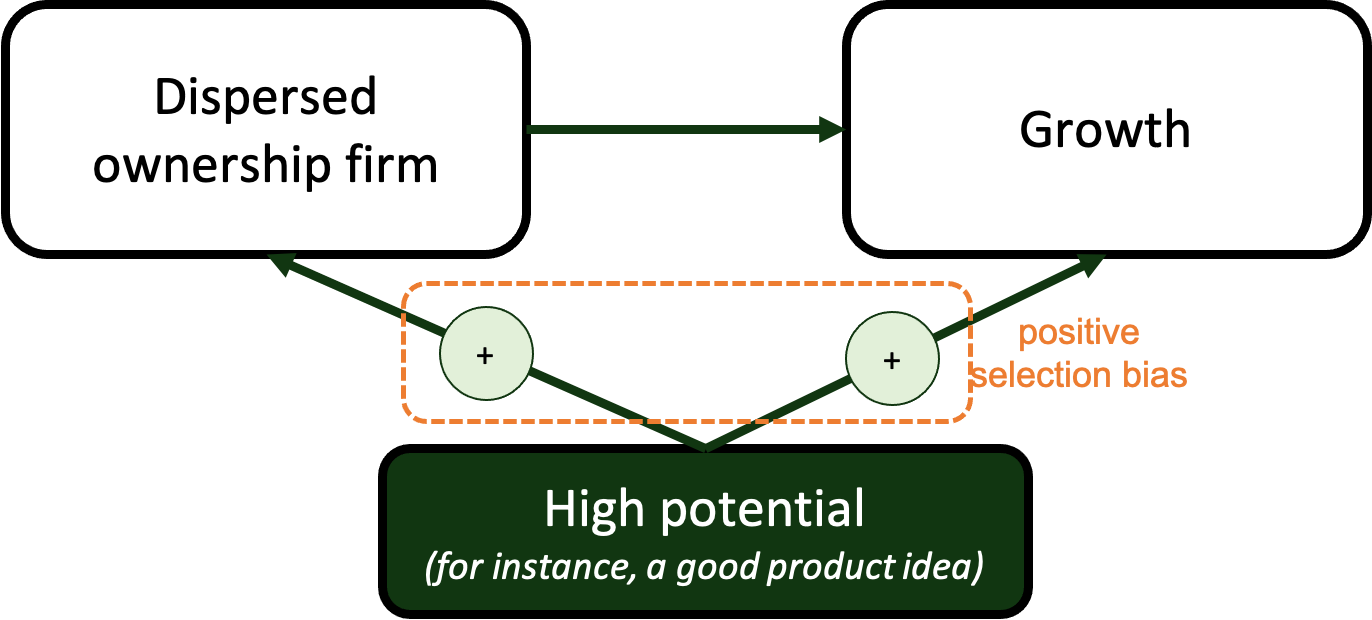
\includegraphics[width=0.8\textwidth]{selectionQ1.png}
\end{figure}

Remember, the observed difference is $\mathbb{E}\left[\textcolor{red}{Y_{i} \mid D_{i}=1}\right]-\mathbb{E}\left[\textcolor{red}{Y_{i} \mid D_{i}=0}\right] = $ \\ 
    $ \underbrace{\mathbb{E}\left[\textcolor{red}{Y_{1 i} \mid D_{i}=1}\right]-\mathbb{E}\left[Y_{0 i} \mid D_{i}=1\right]}_{\text {average effect on dispersed firms (= 0)}} + \underbrace{\mathbb{E}\left[Y_{0 i} \mid D_{i}=1\right]-\mathbb{E}\left[\textcolor{red}{Y_{0 i} \mid D_{i}=0}\right]}_{\text {selection bias } (> 0)} $

\end{frame}

\begin{frame}{Problem set - Question 1.}

What is the effect of studying economics rather than sociology on the salaries of university graduates?

\begin{itemize}
    \item (a) Outcome and treatment?
    \item (b) Counterfactual outcomes.
    \item (c) Causal channels?
    \item (d) Possible sources of selection bias.
\end{itemize}
\end{frame}

\begin{frame}{Problem set - Question 1.}

What is the effect of studying economics rather than sociology on the salaries of university graduates?

\begin{itemize}
    \item (a) \alert{Outcome and treatment?}
    \begin{itemize}
        \item \alert{$Y_i =$ salary, $D_i=$ studying economics}
    \end{itemize}
    \item (b) Counterfactual outcomes.
    \item (c) Causal channels?
    \item (d) Possible sources of selection bias.
\end{itemize}
\end{frame}

\begin{frame}{Problem set - Question 1.}

What is the effect of studying economics rather than sociology on the salaries of university graduates?

\begin{itemize}
    \item (a) Outcome and treatment?
    \item \alert{(b) Counterfactual outcomes.}
    \begin{itemize}
        \item \alert{$Y_{0i} =$ salary of $i$ if $i$ studies sociology}
        \item \alert{$Y_{1i} =$ salary of $i$ if $i$ studies economics}
    \end{itemize}
    \item (c) Causal channels?
    \item (d) Possible sources of selection bias.
\end{itemize}
\end{frame}

\begin{frame}{Problem set - Question 1.}

What is the effect of studying economics rather than sociology on the salaries of university graduates?

\begin{itemize}
    \item (a) Outcome and treatment?
    \item (b) Counterfactual outcomes.
    \item (c) Causal channels?
    \item (d) Possible sources of selection bias.
\end{itemize}
\end{frame}

\end{document}